%% BioMed_Central_Tex_Template_v1.06
%%                                      %
%  bmc_article.tex            ver: 1.06 %
%                                       %

%%IMPORTANT: do not delete the first line of this template
%%It must be present to enable the BMC Submission system to
%%recognise this template!!

%%%%%%%%%%%%%%%%%%%%%%%%%%%%%%%%%%%%%%%%%
%%                                     %%
%%  LaTeX template for BioMed Central  %%
%%     journal article submissions     %%
%%                                     %%
%%          <8 June 2012>              %%
%%                                     %%
%%                                     %%
%%%%%%%%%%%%%%%%%%%%%%%%%%%%%%%%%%%%%%%%%


%%%%%%%%%%%%%%%%%%%%%%%%%%%%%%%%%%%%%%%%%%%%%%%%%%%%%%%%%%%%%%%%%%%%%
%%                                                                 %%
%% For instructions on how to fill out this Tex template           %%
%% document please refer to Readme.html and the instructions for   %%
%% authors page on the biomed central website                      %%
%% http://www.biomedcentral.com/info/authors/                      %%
%%                                                                 %%
%% Please do not use \input{...} to include other tex files.       %%
%% Submit your LaTeX manuscript as one .tex document.              %%
%%                                                                 %%
%% All additional figures and files should be attached             %%
%% separately and not embedded in the \TeX\ document itself.       %%
%%                                                                 %%
%% BioMed Central currently use the MikTex distribution of         %%
%% TeX for Windows) of TeX and LaTeX.  This is available from      %%
%% http://www.miktex.org                                           %%
%%                                                                 %%
%%%%%%%%%%%%%%%%%%%%%%%%%%%%%%%%%%%%%%%%%%%%%%%%%%%%%%%%%%%%%%%%%%%%%

%%% additional documentclass options:
%  [doublespacing]
%  [linenumbers]   - put the line numbers on margins

%%% loading packages, author definitions

\documentclass[twocolumn]{bmcart}% uncomment this for twocolumn layout and comment line below
% \documentclass{bmcart}

%%% Load packages
\usepackage{amsthm,amsmath}
\RequirePackage{natbib}
%\RequirePackage[authoryear]{natbib}% uncomment this for author-year bibliography
\RequirePackage{hyperref}
\usepackage[utf8]{inputenc} %unicode support
%\usepackage[applemac]{inputenc} %applemac support if unicode package fails
%\usepackage[latin1]{inputenc} %UNIX support if unicode package fails
\usepackage{lineno} % for line numbers
\usepackage{textcomp} % for single quotes
% orcid code from https://tex.stackexchange.com/questions/445563/ieeetran-how-to-include-orcid-in-tex-pdf-with-pdflatex/445583#445583
\usepackage{scalerel}
\usepackage{tikz}
\usetikzlibrary{svg.path}

\definecolor{orcidlogocol}{HTML}{A6CE39}
\tikzset{
    orcidlogo/.pic={
        \fill[orcidlogocol] svg{M256,128c0,70.7-57.3,128-128,128C57.3,256,0,198.7,0,128C0,57.3,57.3,0,128,0C198.7,0,256,57.3,256,128z};
        \fill[white] svg{M86.3,186.2H70.9V79.1h15.4v48.4V186.2z}
        svg{M108.9,79.1h41.6c39.6,0,57,28.3,57,53.6c0,27.5-21.5,53.6-56.8,53.6h-41.8V79.1z M124.3,172.4h24.5c34.9,0,42.9-26.5,42.9-39.7c0-21.5-13.7-39.7-43.7-39.7h-23.7V172.4z}
        svg{M88.7,56.8c0,5.5-4.5,10.1-10.1,10.1c-5.6,0-10.1-4.6-10.1-10.1c0-5.6,4.5-10.1,10.1-10.1C84.2,46.7,88.7,51.3,88.7,56.8z};
    }
}

\newcommand\orcidicon[1]{\href{https://orcid.org/#1}{\mbox{\scalerel*{
                
\begin{tikzpicture}[yscale=-1,transform shape]
                \pic{orcidlogo};
                \end{tikzpicture}
            }{|}}}}

\usepackage{lineno}
\usepackage{textcomp}
\usepackage{enumitem}
\usepackage{hyperref} %<--- Load after everything else

%%%%%%%%%%%%%%%%%%%%%%%%%%%%%%%%%%%%%%%%%%%%%%%%%
%%                                             %%
%%  If you wish to display your graphics for   %%
%%  your own use using includegraphic or       %%
%%  includegraphics, then comment out the      %%
%%  following two lines of code.               %%
%%  NB: These line *must* be included when     %%
%%  submitting to BMC.                         %%
%%  All figure files must be submitted as      %%
%%  separate graphics through the BMC          %%
%%  submission process, not included in the    %%
%%  submitted article.                         %%
%%                                             %%
%%%%%%%%%%%%%%%%%%%%%%%%%%%%%%%%%%%%%%%%%%%%%%%%%


\def\includegraphic{}
\def\includegraphics{}

\providecommand{\tightlist}{%
  \setlength{\itemsep}{0pt}\setlength{\parskip}{0pt}}

%%% Put your definitions there:
\startlocaldefs
\usepackage{url}
\endlocaldefs
\providecommand{\tightlist}{%
  \setlength{\itemsep}{0pt}\setlength{\parskip}{0pt}}

%%% Begin ...
\begin{document}

%%% Start of article front matter
\begin{frontmatter}

\begin{fmbox}
\dochead{Educational}

%%%%%%%%%%%%%%%%%%%%%%%%%%%%%%%%%%%%%%%%%%%%%%
%%                                          %%
%% Enter the title of your article here     %%
%%                                          %%
%%%%%%%%%%%%%%%%%%%%%%%%%%%%%%%%%%%%%%%%%%%%%%

\title{Intuitive, reproducible high-throughput molecular dynamics in Galaxy: a tutorial}

%%%%%%%%%%%%%%%%%%%%%%%%%%%%%%%%%%%%%%%%%%%%%%
%%                                          %%
%% Enter the authors here                   %%
%%                                          %%
%% Specify information, if available,       %%
%% in the form:                             %%
%%   <key>={<id1>,<id2>}                    %%
%%   <key>=                                 %%
%% Comment or delete the keys which are     %%
%% not used. Repeat \author command as much %%
%% as required.                             %%
%%                                          %%
%%%%%%%%%%%%%%%%%%%%%%%%%%%%%%%%%%%%%%%%%%%%%%

\author[ addressref={aff1},                   % id's of addresses, e.g. {aff1,aff2}
   noteref={n1},                        % id's of article notes, if any
   email={sbray1371@gmail.com}   % email address
]{\inits{SAB}\fnm{Simon A} \snm{Bray}} \orcidicon{0000-0002-0621-6705}
\author[
   addressref={aff2},
   noteref={n1},
   email={}
]{\inits{TS}\fnm{Tharindu} \snm{Senapathi}} \orcidicon{0000-0002-3277-4022}
\author[
   addressref={aff2},
   email={chris.barnett@uct.ac.za}
]{\inits{CB}\fnm{Christopher B} \snm{Barnett}} \orcidicon{0000-0002-1467-5741}
\author[
   addressref={aff1},
   corref={aff1},
   email={gruening@informatik.uni-freiburg.de}
]{\inits{BG}\fnm{Björn} \snm{Grüning}} \orcidicon{0000-0002-3079-6586}
\author[
   addressref={aff2},
   email={kevin.naidoo@uct.ac.za}
]{\inits{KJ}\fnm{Kevin J} \snm{Naidoo}} \orcidicon{0000-0002-9898-3708}

%%%%%%%%%%%%%%%%%%%%%%%%%%%%%%%%%%%%%%%%%%%%%%
%%                                          %%
%% Enter the authors' addresses here        %%
%%                                          %%
%% Repeat \address commands as much as      %%
%% required.                                %%
%%                                          %%
%%%%%%%%%%%%%%%%%%%%%%%%%%%%%%%%%%%%%%%%%%%%%%

\address[id=aff1]{%                           % unique id
   \orgname{Department of Computer Science, University of Freiburg}, % university, etc
   \street{Georges-Köhler-Allee 106},                     %
  %\postcode{}                                % post or zip code
   \city{Freiburg},                              % city
   \cny{Germany}                                    % country
}
\address[id=aff2]{%
  \orgname{Scientific Computing Research Unit, University of Cape Town},
  \postcode{7700}
  \city{Cape Town},
  \cny{South Africa}
}



%%%%%%%%%%%%%%%%%%%%%%%%%%%%%%%%%%%%%%%%%%%%%%
%%                                          %%
%% Enter short notes here                   %%
%%                                          %%
%% Short notes will be after addresses      %%
%% on first page.                           %%
%%                                          %%
%%%%%%%%%%%%%%%%%%%%%%%%%%%%%%%%%%%%%%%%%%%%%%

\begin{artnotes}
%\note{Sample of title note}     % note to the article
\note[id=n1]{Equal contributor} % note, connected to author
\end{artnotes}

\end{fmbox}% comment this for two column layout

%%%%%%%%%%%%%%%%%%%%%%%%%%%%%%%%%%%%%%%%%%%%%%
%%                                          %%
%% The Abstract begins here                 %%
%%                                          %%
%% Please refer to the Instructions for     %%
%% authors on http://www.biomedcentral.com  %%
%% and include the section headings         %%
%% accordingly for your article type.       %%
%%                                          %%
%%%%%%%%%%%%%%%%%%%%%%%%%%%%%%%%%%%%%%%%%%%%%%

\begin{abstractbox}

\begin{abstract} % abstract
This paper is a tutorial developed for the data analysis platform Galaxy. The
Galaxy's concept makes high-throughput computational data analysis a
structured, reproducible and transparent process. In this tutorial we
focus on 3 questions: How are protein-ligand systems parameterized for
molecular dynamics simulation? What kind of analysis can be carried out
on molecular trajectories? How can high-throughput MD be used to study
multiple ligands? After finishing you will be able to learn about
force-fields and MD parameterization, learn how to conduct MD simulation
and analysis for a protein-ligand system, understand how different
molecular interactions contribute to the binding affinity of various
ligands for the Hsp90 protein. Requirements for this tutorial is a
minimal Galaxy experience and a Galaxy account on the Galaxy Europe
server. The estimated duration of this tutorial is around 3 hours.

\end{abstract}

%%%%%%%%%%%%%%%%%%%%%%%%%%%%%%%%%%%%%%%%%%%%%%
%%                                          %%
%% The keywords begin here                  %%
%%                                          %%
%% Put each keyword in separate \kwd{}.     %%
%%                                          %%
%%%%%%%%%%%%%%%%%%%%%%%%%%%%%%%%%%%%%%%%%%%%%%

\begin{keyword}
\kwd{Galaxy}
\kwd{Molecular Dynamics}
\kwd{Repeatable}
\end{keyword}

% MSC classifications codes, if any
%\begin{keyword}[class=AMS]
%\kwd[Primary ]{}
%\kwd{}
%\kwd[; secondary ]{}
%\end{keyword}

\end{abstractbox}
%
%\end{fmbox}% uncomment this for twcolumn layout

\end{frontmatter}

%%%%%%%%%%%%%%%%%%%%%%%%%%%%%%%%%%%%%%%%%%%%%%
%%                                          %%
%% The Main Body begins here                %%
%%                                          %%
%% Please refer to the instructions for     %%
%% authors on:                              %%
%% http://www.biomedcentral.com/info/authors%%
%% and include the section headings         %%
%% accordingly for your article type.       %%
%%                                          %%
%% See the Results and Discussion section   %%
%% for details on how to create sub-sections%%
%%                                          %%
%% use \cite{...} to cite references        %%
%%  \cite{koon} and                         %%
%%  \cite{oreg,khar,zvai,xjon,schn,pond}    %%
%%  \nocite{smith,marg,hunn,advi,koha,mouse}%%
%%                                          %%
%%%%%%%%%%%%%%%%%%%%%%%%%%%%%%%%%%%%%%%%%%%%%%

%%%%%%%%%%%%%%%%%%%%%%%%% start of article main body
% <put your article body there>

%%%%%%%%%%%%%%%%
%% Background %%
%%


%\linenumbers

\hypertarget{introduction}{%
\section*{Introduction}\label{introduction}}

Molecular dynamics (MD) ... However, the barrier to entry for MD simulation is high; not only is the theory difficult to master, but commonly used MD software is technically demanding. Furthermore, generating reliable, reproducible simulation data requires the user to maintain detailed records of all parameters and files used, which again poses a challenge to newcomers to the field. One solution to the latter problem is usage of a workflow management system such as Galaxy, KNIME or CWL; both the former provide molecular dynamics tools/nodes.

This tutorial provides a detailed workflow for high-throughput molecular dynamics using Galaxy. Galaxy
\cite{afgan2018galaxy} is a data analysis platform that provides access to thousands of tools for scientific computation. It features a web-based user interface while automatically and transparently managing underlying computation details. Galaxy's
concept makes high-throughput sequencing data analysis a structured, reproducible and transparent process.

The aim of this tutorial is to guide the user through the various steps of a molecular dynamics study, from accessing publicly available crystal structures, to performing MD simulation (leveraging the popular GROMACS engine), to analysis of the results.

The entire analysis described this article can be conducted efficiently on any Galaxy server which has the needed tools. In particular, we recommend using the Galaxy Europe server
(\url{https://cheminformatics.usegalaxy.eu/}) or the Galaxy South Africa server (\url{https://galaxy-compchem.ilifu.ac.za/}).

The tutorial presented in this article has been developed by the Galaxy Training Network \cite{batut2018community} and its most up-to-date
version is available online on the \href{https://training.galaxyproject.org/topics/computational-chemistry/tutorials/htmd-analysis/tutorial.html}{Galaxy Training Materials} website.

This tutorial provides an introduction to using high-throughput
molecular dynamics to study protein-ligand interaction, as applied to
N-terminus of Hsp90 (heat shock protein 90).

\subsection*{What is high-throughput molecular
dynamics?}\label{what-is-high-throughput-molecular-dynamics}

Molecular dynamics (MD) is a method to simulate molecular motion by
iterative application of Newton's laws of motion. It is often applied to
large biomolecules such as proteins or nucleic acids. A common
application is to assess the interaction between these macromolecules
and a number of small molecules (e.g.~potential drug candidates). This
tutorial provides a guide to setting up and running a high-throughput
workflow for screening multiple small molecules, using the open-source
GROMACS tools provided through the Galaxy platform.

\subsection*{Why is Hsp90 interesting to
study?}\label{why-is-hsp90-interesting-to-study}

The 90 kDa heat shock protein (Hsp90) is a chaperone protein responsible
for catalyzing the conversion of a wide variety of proteins to a
functional form; examples of the Hsp90 clientele, which totals several
hundred proteins, include nuclear steroid hormone receptors and protein
kinases. The mechanism by which Hsp90 acts varies between clients, as
does the client binding site; the process is dependent on
post-translational modifications of Hsp90 and the identity of
co-chaperones which bind and regulate the conformational cycle.

Due to its vital biochemical role as a chaperone protein involved in
facilitating the folding of many client proteins, Hsp90 is an attractive
pharmaceutical target. In particular, as protein folding is a potential
bottleneck to slow cellular reproduction and growth, blocking Hsp90
function using inhibitors which bind tightly to the ATP binding site
could assist in treating cancer; for example, the antibiotic
geldanamycin and its analogs are under investigation as possible
anti-tumor agents.



\hypertarget{methods}{%
\section*{Methods}\label{simulation}}
\hypertarget{simulation}{%
\section*{Simulation}\label{simulation}}

\subsection{Get data}\label{get-data}}

First of all, download the required data.

\textbf{\emph{Hands-on: Data upload}}

\begin{enumerate}
\def\labelenumi{\arabic{enumi}.}
\tightlist
\item
  Create a new history for this tutorial

\item
  Rename the dataset to `Hsp90 structure'
\item
  Search Galaxy for the 'Get PDB' tool. Request the accession code \texttt{6hhr}.
\item
  Check that the datatype is correct (PDB file).
\end{enumerate}

\subsection{Topology generation}\label{topology-generation}

Now we have downloaded a PDB structure of the protein we wish to study, we will start parameterizing it for MD simulation.

GROMACS distinguishes between constant and dynamic attributes of the
atoms in the system. The constant attributes (e.g. atom charges, bonds
connecting atoms) are listed in the topology (TOP file), while dynamic
attributes (attributes that can change during a simulation, e.g. atom
position, velocities and forces) are stored in structure (PDB or GRO)
and trajectory (XTC and TRR) files.

The PDB file we start from only explicitly states atom type and
position. Therefore, before beginning simulation, we need to calculate
the rest of the information contained within the topology file. There
are a range of force fields which perform these calculations in slightly
different ways.

% perhaps some more discussion here and a citation of https://www.sciencedirect.com/science/article/pii/S1877117319302157

Parameterization needs to be done separately for the ligand and protein.
Therefore, the first step is to separate the PDB file into two sets of
coordinates - one for the ligand and one for the protein.

\subsubsection{Extract protein and ligand
coordinates}\label{extract-protein-and-ligand-coordinates}



\begin{quote}
\subsubsection{Hands-on: Task
description}\label{hands-on-task-description}

\begin{enumerate}
\def\labelenumi{\arabic{enumi}.}
\tightlist
\item
  \textbf{Search in textfiles} with the following parameters:
  \begin{itemize}
  \tightlist
  \item
    \emph{``Select lines from''}: `Hsp90 structure'\\
  \item
    \emph{``that''}: \texttt{Don\textquotesingle{}t\ Match}
  \item
    \emph{``Regular Expression''}: \texttt{HETATM}
  \end{itemize}
\item
  Rename output to `Protein (PDB)'
\item
  \textbf{Search in textfiles} with the following parameters:

  \begin{itemize}
  \tightlist
  \item
    \emph{``Select lines from''}: `Hsp90 structure'\\
  \item
    \emph{``that''}: \texttt{Match}
  \item
    \emph{``Regular Expression''}: \texttt{AG5E}
  \end{itemize}
\item
  Rename output to `Ligand (PDB)'
\end{enumerate}


\end{quote}

\hypertarget{set-up-protein-topology}{%
\subsubsection{Set up protein topology}\label{set-up-protein-topology}}

Firstly, we need to calculate the topology for the protein file. We will
use the \textbf{GROMACS initial setup} tool.

\begin{quote}
\subsubsection{Hands-on: Task
description}\label{hands-on-task-description-1}

\begin{enumerate}
\def\labelenumi{\arabic{enumi}.}
\tightlist
\item
  \textbf{GROMACS initial setup} with the following parameters:

  \begin{itemize}
  \tightlist
  \item
    \emph{``PDB input file''}: `Protein (PDB)' file
  \item
    \emph{``Force field''}: \texttt{gaff}
  \item
    \emph{``Water model''}: \texttt{TIP3P}
  \item
    \emph{``Generate detailed log''}: \texttt{Yes}
  \end{itemize}
\end{enumerate}


\end{quote}

The tool produces four outputs: a GRO file (containing the coordinates
of the protein), a TOP file (containing other information, including on
charges, masses, bonds and angles), an ITP file (which will be used to
restrain the protein position in the equilibration step later on), and a
log for the tool.

Please note all GROMACS tools output a log. Generally, you only need to
look at this when a job fails. It provides useful information for
debugging if we encounter any problems.

\subsubsection{Generate a topology for the
ligand}\label{generate-a-topology-for-the-ligand}

To generate a topology for the ligand, we will use the \textbf{acpype}
tool. This provides a convenient interface to the AmberTools suite and
allows us to easily create the ligand topology in the format required by
GROMACS.

\begin{quote}
\subsubsection{Hands-on: Task
description}\label{hands-on-task-description-2}

\begin{enumerate}
\def\labelenumi{\arabic{enumi}.}
\tightlist
\item
  \textbf{Generate MD topologies for small molecules} with the following
  parameters:

  \begin{itemize}
  \tightlist
  \item
    \emph{``Input file''}: `Ligand (PDB)'
  \item
    \emph{``Charge of the molecule''}: \texttt{0}
  \item
    \emph{``Multiplicity''}: \texttt{1}
  \item
    \emph{``Force field to use for parameterization''}:
    \texttt{AMBER14SB}
  \item
    \emph{``Save GRO file?''}: \texttt{Yes}
  \end{itemize}
\end{enumerate}

\end{quote}

\subsection{Solvation and energy
minimization}\label{solvation-and-energy-minimization}

Having generated topologies, we now need to combine them, define the box
which contains the system, add solvent and ions, and perform an energy
minimization step.

\subsubsection{Combine topology and GRO
files}\label{combine-topology-and-gro-files}

\begin{quote}
\subsubsection{Hands-on: Combine GRO
files}\label{hands-on-combine-gro-files}

\begin{enumerate}
\def\labelenumi{\arabic{enumi}.}
\tightlist
\item
  On the \texttt{Structure\ file\ (GRO\ format)} created by the
  \textbf{acpype} tool,click on the \texttt{Visualize\ this\ data} icon.
  Select \texttt{Editor} to open the file using the text editor
  integrated into Galaxy. Select all the lines starting with
  \texttt{1\ GSE} and copy your selection.
\item
  Open the Protein GRO file by clicking on the
  \texttt{Visualize\ this\ data} button on the dataset.
\item
  Paste the lines from the ligand GRO file just before the last line.
\item
  If you scroll back to the top, you will see that the total number of
  atoms in the system is given in the second line (\texttt{3280}). You
  have just added 21 new atoms, so increase the value by 21 to
  \texttt{3301}.
\item
  Click \texttt{Export} to save your changes as a new dataset. Make sure
  the datatype of the new file is still \texttt{GRO}. Rename to
  \texttt{System\ GRO\ file}.
\end{enumerate}
\end{quote}

\begin{quote}
\subsubsection{Hands-on: Combine topology
files}\label{hands-on-combine-topology-files}

\begin{enumerate}
\def\labelenumi{\arabic{enumi}.}
\tightlist
\item
  On the ligand \texttt{Topology} created by the \textbf{acpype} tool,
  right-click on the \texttt{Visualize\ this\ data} icon and open the
  link in a new tab. Select the first section in the file, starting with
  \texttt{{[}\ atomtypes\ {]}}, and copy the selection.
\item
  Returning to the first tab, open the protein TOP file using the text
  editor integrated into Galaxy by clicking on the
  \texttt{Visualize\ this\ data} button on the dataset.
\item
  Paste the lines from the ligand ITP file near to the top of the file,
  just after the line \texttt{\#include\ "amber99sb.ff/forcefield.itp"}.
\item
  Go back to the ligand ITP file and select the rest of the file (from
  \texttt{{[}\ moleculetypes\ {]}}) onwards. Copy the selection.
\item
  In the protein TOP file, paste the selection near to the bottom of the
  file, before the line \texttt{;\ Include\ water\ topology} (and just
  after the position restraint file). Notice that the
  \texttt{{[}\ moleculetype\ {]}} section you just copied starts with
  \texttt{base} - this is the name acpype has given to the ligand. Feel
  free to change this to whatever you prefer - \texttt{ligand}, or
  \texttt{GSE}.
\item
  Finally, we need to state in the topology that we have included a new
  kind of molecule. Go to the final section
  (\texttt{{[}\ molecules\ {]}}) and add a new line \texttt{base} (or
  whatever name you gave the ligand in step 5), with a 1 in the
  \texttt{\#mols} column.
\item
  Click \texttt{Export} to save your changes as a new dataset. Make sure
  the datatype of the new file is still \texttt{TOP}. Rename to
  \texttt{System\ topology}.
\end{enumerate}
\end{quote}

If this procedure was too complicated, you can download the combined
files here: LINK. However, you will find it useful to understand the
information contained within topology files and learn how to make
changes to it.

% needs updating with the new tool

\subsubsection{\texorpdfstring{Create the simulation box with
\textbf{GROMACS structure
configuration}}{Create the simulation box with GROMACS structure configuration}}\label{create-the-simulation-box-with-gromacs-structure-configuration}

The next step, once combined coordinate (GRO) and topology (TOP) files
have been created, is to create a simulation box in which the system is
situated.

\begin{quote}
\hypertarget{hands-on-task-description-3}{%
\subsubsection{Hands-on: Task
description}\label{hands-on-task-description-3}}

\begin{enumerate}
\def\labelenumi{\arabic{enumi}.}
%\tightlist
\item
  \textbf{GROMACS structure configuration} with the following
  parameters:

  \begin{itemize}
%  \tightlist
  \item
    \emph{``Input structure''}: \texttt{System\ GRO\ file} (Input
    dataset)
  \item
    \emph{``Configure box?''}: \texttt{Yes}

    \begin{itemize}
%    \tightlist
    \item
      \emph{``Box dimensions in nanometers''}: \texttt{1.0}
    \item
      \emph{``Box type''}: \texttt{Triclinic}
    \end{itemize}
  \item
    \emph{``Generate detailed log''}: \texttt{Yes}
  \end{itemize}
\end{enumerate}

\end{quote}

\subsubsection{Solvation}\label{solvation}
The next step is solvation of the newly created simulation box. Note
that the system is charged (depending on the pH) - the solvation tool
also adds sodium or chloride ions as required to neutralise this.

\begin{quote}
\subsubsection{Hands-on: Task
description}\label{hands-on-task-description-4}

\begin{enumerate}
\def\labelenumi{\arabic{enumi}.}
\tightlist
\item
  \textbf{GROMACS solvation and adding ions} with the following
  parameters:

  \begin{itemize}
  \tightlist
  \item
    \emph{``GRO structure file''}: \texttt{output} (output of
    \textbf{GROMACS structure configuration} )
  \item
    \emph{``System topology''}: \texttt{output}
  \item
    \emph{``Generate detailed log''}: \texttt{Yes}
  \end{itemize}
\end{enumerate}

\end{quote}

\subsubsection{Energy minimization}\label{energy-minimization}

The next step is energy minimization, which can be carried out using the
\textbf{GROMACS energy minimization} tool.

\begin{quote}
\subsubsection{Hands-on: Task
description}\label{hands-on-task-description-5}

\begin{enumerate}
\def\labelenumi{\arabic{enumi}.}
\tightlist
\item
  \textbf{GROMACS energy minimization} with the following parameters:

  \begin{itemize}
  \tightlist
  \item
    \emph{``GRO structure file.''}: \texttt{output1} (output of
    \textbf{GROMACS solvation and adding ions} )
  \item
    \emph{``Topology (TOP) file.''}: \texttt{output2} (output of
    \textbf{GROMACS solvation and adding ions} )
  \item
    \emph{``Parameter input''}:
    \texttt{Use\ default\ (partially\ customisable)\ setting}

    \begin{itemize}
    \tightlist
    \item
      \emph{``Number of steps for the MD simulation''}: \texttt{50000}
    \item
      \emph{``EM tolerance''}: \texttt{1000.0}
    \end{itemize}
  \item
    \emph{``Generate detailed log''}: \texttt{Yes}
  \item
    Rename output to \texttt{Minimized\ GRO\ file}
  \end{itemize}
\end{enumerate}

\end{quote}

\subsection{Equilibration}\label{equilibration}

We now carry out equilibration in two stages: NVT and NPT. This is
discussed at greater length in the basic GROMACS tutorial. Equilibration
requires restraining the protein structure - we use the ITP file
produced by the initial setup tool for this.

\begin{quote}
\subsubsection{Hands-on: NVT
equilibration}\label{hands-on-nvt-equilibration}

\begin{enumerate}
\def\labelenumi{\arabic{enumi}.}
\tightlist
\item
  \textbf{GROMACS simulation} with the following parameters:

  \begin{itemize}
  \tightlist
  \item
    \emph{``GRO structure file''}: \texttt{Minimized\ GRO\ file} (from
    energy minimization step)
  \item
    \emph{``Topology (TOP) file''}: TOP file produced by solvation step.
  \item
    In \emph{``Inputs''}:

    \begin{itemize}
    \tightlist
    \item
      \emph{``Position restraint (ITP) file''}: ITP file produced by
      initial setup step.
    \end{itemize}
  \item
    In \emph{``Outputs''}:

    \begin{itemize}
    \tightlist
    \item
      \emph{``Trajectory output''}:
      \texttt{Return\ .xtc\ file\ (reduced\ precision)}
    \item
      \emph{``Structure output''}: \texttt{Return\ .gro\ file}
    \item
      \emph{``Produce a checkpoint (CPT) file''}:
      \texttt{Produce\ CPT\ output}
    \end{itemize}
  \item
    In \emph{``Settings''}:

    \begin{itemize}
    \tightlist
    \item
      \emph{``Parameter input''}:
      \texttt{Use\ default\ (partially\ customisable)\ setting}

      \begin{itemize}
      \tightlist
      \item
        \emph{``Bond constraints (constraints)''}:
        \texttt{All\ bonds\ (all-bonds).}
      \item
        \emph{``Temperature /K''}: \texttt{300}
      \item
        \emph{``Step length in ps''}: \texttt{0.0002}
      \item
        \emph{``Number of steps that elapse between saving data points
        (velocities, forces, energies)''}: \texttt{1000}
      \item
        \emph{``Number of steps for the simulation''}: \texttt{50000}
      \end{itemize}
    \end{itemize}
  \item
    \emph{``Generate detailed log''}: \texttt{Yes}
  \end{itemize}
\end{enumerate}

\end{quote}

Having stabilized the temperature of the system with NVT equilibration,
we also need to stabilize the pressure of the system. We therefore
equilibrate again using the NPT (constant number of particles, pressure,
temperature) ensemble.

Note that we can continue where the last simulation left off (with new
parameters) by using the checkpoint (CPT) file saved at the end of the
NVT simulation.

\begin{quote}
\subsubsection{Hands-on: NPT
equilibration}\label{hands-on-npt-equilibration}

\begin{enumerate}
\def\labelenumi{\arabic{enumi}.}
\tightlist
\item
  \textbf{GROMACS simulation} with the following parameters:

  \begin{itemize}
  \tightlist
  \item
    \emph{``GRO structure file''}: GRO output of \textbf{GROMACS
    simulation} (NVT equilibration)
  \item
    \emph{``Topology (TOP) file''}: TOP file produced by solvation step.
  \item
    In \emph{``Inputs''}:

    \begin{itemize}
    \tightlist
    \item
      \emph{``Checkpoint (CPT) file''}: Output of \textbf{GROMACS
      simulation} (NVT equilibration))
    \item
      \emph{``Position restraint (ITP) file''}: ITP file produced by
      initial setup step.
    \end{itemize}
  \item
    In \emph{``Outputs''}:

    \begin{itemize}
    \tightlist
    \item
      \emph{``Trajectory output''}:
      \texttt{Return\ .xtc\ file\ (reduced\ precision)}
    \item
      \emph{``Structure output''}: \texttt{Return\ .gro\ file}
    \item
      \emph{``Produce a checkpoint (CPT) file''}:
      \texttt{Produce\ CPT\ output}
    \end{itemize}
  \item
    In \emph{``Settings''}:

    \begin{itemize}
    \tightlist
    \item
      \emph{``Ensemble''}: \texttt{Isothermal-isobaric\ ensemble\ (NPT)}
    \item
      \emph{``Parameter input''}:
      \texttt{Use\ default\ (partially\ customisable)\ setting}

      \begin{itemize}
      \tightlist
      \item
        \emph{``Bond constraints (constraints)''}:
        \texttt{All\ bonds\ (all-bonds).}
      \item
        \emph{``Temperature /K''}: \texttt{300}
      \item
        \emph{``Step length in ps''}: \texttt{0.002}
      \item
        \emph{``Number of steps that elapse between saving data points
        (velocities, forces, energies)''}: \texttt{1000}
      \item
        \emph{``Number of steps for the simulation''}: \texttt{50000}
      \end{itemize}
    \end{itemize}
  \item
    \emph{``Generate detailed log''}: \texttt{Yes}
  \end{itemize}
\end{enumerate}

\end{quote}

\subsection{Main simulation}\label{main-simulation}

We can now remove the restraints and continue with the simulation. The
simulation will run for 1 million steps, with a step size of 1 fs, so
wil have a total length of 1 ns.

\begin{quote}
\hypertarget{hands-on-task-description-6}{%
\subsubsection{Hands-on: Task
description}\label{hands-on-task-description-6}}

\begin{enumerate}
\def\labelenumi{\arabic{enumi}.}
\tightlist
\item
  \textbf{GROMACS simulation} with the following parameters:

  \begin{itemize}
  \tightlist
  \item
    \emph{``GRO structure file''}: Output of \textbf{GROMACS simulation}
    (NPT equilibration)
  \item
    \emph{``Topology (TOP) file''}: Output of the solvation step
  \item
    In \emph{``Inputs''}:

    \begin{itemize}
    \tightlist
    \item
      \emph{``Checkpoint (CPT) file''}: Output of \textbf{GROMACS
      simulation} (NPT simulation))
    \end{itemize}
  \item
    In \emph{``Outputs''}:

    \begin{itemize}
    \tightlist
    \item
      \emph{``Trajectory output''}:
      \texttt{Return\ .xtc\ file\ (reduced\ precision)}
    \item
      \emph{``Structure output''}: \texttt{Return\ .gro\ file}
    \item
      \emph{``Produce a checkpoint (CPT) file''}:
      \texttt{Produce\ CPT\ output}
    \end{itemize}
  \item
    In \emph{``Settings''}:

    \begin{itemize}
    \tightlist
    \item
      \emph{``Ensemble''}: \texttt{Isothermal-isobaric\ ensemble\ (NPT)}
    \item
      \emph{``Parameter input''}:
      \texttt{Use\ default\ (partially\ customisable)\ setting}

      \begin{itemize}
      \tightlist
      \item
        \emph{``Temperature /K''}: \texttt{300}
      \item
        \emph{``Step length in ps''}: \texttt{0.001}
      \item
        \emph{``Number of steps that elapse between saving data points
        (velocities, forces, energies)''}: \texttt{1000}
      \item
        \emph{``Number of steps for the simulation''}: \texttt{1000000}
      \end{itemize}
    \end{itemize}
  \item
    \emph{``Generate detailed log''}: \texttt{Yes}
  \end{itemize}
\end{enumerate}

\end{quote}

\hypertarget{analysis}{%
\subsection*{Analysis}\label{analysis}}

An analysis of the GROMACS simulation outputs will be carried out using Galaxy tools developed for computational chemistry\cite{senapathi_biomolecular_2019} based on popular analysis software - MDAnalysis\cite{michaudagrawal_mdanalysis_2011}, MDTraj\cite{mcgibbon_mdtraj_2015} and Bio3D\cite{skjaerven_integrating_2014}. See figure \ref{fig:analysisworkflow} for an overview of the workflow.

\begin{figure}[h!]
\caption{\csentence{Analysis workflow.}
    Analysis workflow for Hsp90 with ligand}
\centering
\label{fig:analysisworkflow}
\end{figure}

To check the stability and conformation of the protein and ligand through the course of the simulation RMSD and RMSF are calculated.




\hypertarget{create-pdb-file-needed-by-most-analysis-tools}{%
\subsubsection{Create PDB file needed by most analysis
tools}\label{create-pdb-file-needed-by-most-analysis-tools}}

Convert the structural coordinates of the system in GRO format into PDB
format. This file will be used by most analysis tools as a starting
structure and ``it contains the topology of the system.''

\begin{quote}

\begin{enumerate}
\def\labelenumi{\arabic{enumi}.}
\tightlist
\item
  \textbf{GROMACS structure configuration} with the following
  parameters:

  \begin{itemize}
  \tightlist
  \item
    \emph{``Output format''}: \texttt{PDB\ file}
  \item
    \emph{``Configure box?''}: \texttt{No}
  \end{itemize}
\end{enumerate}


\end{quote}

\hypertarget{convert-trajectory-to-dcd-format}{%
\subsection{Convert trajectory to DCD
format}\label{convert-trajectory-to-dcd-format}}

Convert from XTC to DCD format. A number of the analysis tools being
used have been built to analyse trajectories in CHARMM's DCD format.

\begin{quote}
\hypertarget{hands-on-task-description-8}{%
\subsubsection{Hands-on: Task
description}\label{hands-on-task-description-8}}

\begin{enumerate}
\def\labelenumi{\arabic{enumi}.}
\tightlist
\item
  \textbf{MDTraj file converter} with the following parameters:

  \begin{itemize}
  \tightlist
  \item
    \emph{``Output format''}: \texttt{DCD\ file} \textgreater{}
  \end{itemize}
\end{enumerate}


\end{quote}

\hypertarget{rmsd-analysis}{%
\subsection{RMSD analysis}\label{rmsd-analysis}}

RMSD is a standard measure of structural distance between coordinate
sets that measures the average distance between a group of atoms. The
RMSD of the C\alpha atoms of the protein backbone is calculated here is and
is a measure of how much the protein has changed between different time
points in the trajectory.

\begin{quote}
\hypertarget{hands-on-task-description-9}{%
\subsubsection{Hands-on: Task
description}\label{hands-on-task-description-9}}

\begin{enumerate}
\def\labelenumi{\arabic{enumi}.}
\tightlist
\item
  \textbf{RMSD Analysis} with the following parameters:

  \begin{itemize}
  \tightlist
  \item
    \emph{``Select domains''}: \texttt{C-alpha}
  \end{itemize}

  \textbf{\emph{TODO}}: \emph{Check parameter descriptions}

  \textbf{\emph{TODO}}: \emph{Consider adding a comment or tip box}
\end{enumerate}


\end{quote}




\begin{quote}
\hypertarget{hands-on-task-description-10}{%
\subsubsection{Hands-on: Task
description}\label{hands-on-task-description-10}}

\begin{enumerate}
\def\labelenumi{\arabic{enumi}.}
\tightlist
\item
  \textbf{RMSD Analysis} with the following parameters:

  \begin{itemize}
  \tightlist
  \item
    \emph{``DCD trajectory input''}: \texttt{output} (output of
    \textbf{MDTraj file converter} )
  \item
    \emph{``PDB input''}: \texttt{output} (output of \textbf{GROMACS
    structure configuration} )
  \item
    \emph{``Select domains''}: \texttt{Ligand}
  \end{itemize}

  \textbf{\emph{TODO}}: \emph{Check parameter descriptions}

  \textbf{\emph{TODO}}: \emph{Consider adding a comment or tip box}
\end{enumerate}


\end{quote}

\begin{quote}
\hypertarget{hands-on-task-description-11}{%
\subsubsection{Hands-on: Task
description}\label{hands-on-task-description-11}}

\begin{enumerate}
\def\labelenumi{\arabic{enumi}.}
\tightlist
\item
  \textbf{RMSD Analysis} with the following parameters:

  \begin{itemize}
  \tightlist
  \item
    \emph{``DCD trajectory input''}: \texttt{output} (output of
    \textbf{MDTraj file converter} )
  \item
    \emph{``PDB input''}: \texttt{output} (output of \textbf{GROMACS
    structure configuration} )
  \item
    \emph{``Select domains''}: \texttt{Residue\ ID}

    \begin{itemize}
    \tightlist
    \item
      \emph{``Residue ID''}: \texttt{UNL}
    \end{itemize}
  \end{itemize}

  \textbf{\emph{TODO}}: \emph{Check parameter descriptions}

  \textbf{\emph{TODO}}: \emph{Consider adding a comment or tip box}
\end{enumerate}


\end{quote}



\hypertarget{rmsf-analysis}{%
\subsection{RMSF analysis}\label{rmsf-analysis}}

The Root Mean Square Fluctuation (RMSF) is valuable to consider as it represents the deviation at a reference position over time. Here, we consider how the fluctuation of particular amino acids in the protein. Depending on the system these fluctuations can be correlated to experimental techniques including Nuclear Magnetic Resonance (NMR) and M\"{o}ssbauer spectrocopy.

\begin{quote}
\hypertarget{hands-on-task-description-12}{%
\subsubsection{Hands-on: Task
description}\label{hands-on-task-description-12}}

\begin{enumerate}
\def\labelenumi{\arabic{enumi}.}
\tightlist
\item
  \textbf{RMSF Analysis} with the following parameters:

  \begin{itemize}
  \tightlist
  \item
    \emph{``DCD trajectory input''}: \texttt{output} (output of
    \textbf{MDTraj file converter} )
  \item
    \emph{``PDB input''}: \texttt{output} (output of \textbf{GROMACS
    structure configuration} )
  \item
    \emph{``Select domains''}: \texttt{C-alpha}
  \end{itemize}

  \textbf{\emph{TODO}}: \emph{Check parameter descriptions}

  \textbf{\emph{TODO}}: \emph{Consider adding a comment or tip box}
\end{enumerate}


\end{quote}


\hypertarget{pca-analysis}{%
\subsection{PCA analysis}\label{pca-analysis}}

Principal component analysis (PCA) converts a set of correlated
observations (movement of all atoms in protein) to a set of principal
components which are linearly independent (or uncorrelated). Here we
will calculate the PCA, visualise it and also calculate the cosine
content.

\begin{quote}
\hypertarget{hands-on-task-description-13}{%
\subsubsection{Hands-on: Task
description}\label{hands-on-task-description-13}}

\begin{enumerate}
\def\labelenumi{\arabic{enumi}.}
\tightlist
\item
  \textbf{PCA} with the following parameters:

  \begin{itemize}
  \tightlist
  \item
    \emph{``DCD trajectory input''}: \texttt{output} (output of
    \textbf{MDTraj file converter} )
  \item
    \emph{``PDB input''}: \texttt{output} (output of \textbf{GROMACS
    structure configuration} )
  \item
    \emph{``Select domains''}: \texttt{C-alpha}
  \end{itemize}

  \textbf{\emph{TODO}}: \emph{Check parameter descriptions}

  \textbf{\emph{TODO}}: \emph{Consider adding a comment or tip box}
\end{enumerate}


\end{quote}



\begin{quote}
\hypertarget{hands-on-task-description-14}{%
\subsubsection{Hands-on: Task
description}\label{hands-on-task-description-14}}

\begin{enumerate}
\def\labelenumi{\arabic{enumi}.}
\tightlist
\item
  \textbf{Cosine Content} with the following parameters:

  \begin{itemize}
  \tightlist
  \item
    \emph{``DCD/XTC trajectory input''}: \texttt{output} (output of
    \textbf{MDTraj file converter} )
  \item
    \emph{``PDB/GRO input''}: \texttt{output} (output of \textbf{GROMACS
    structure configuration} )
  \end{itemize}

  \textbf{\emph{TODO}}: \emph{Check parameter descriptions}

  \textbf{\emph{TODO}}: \emph{Consider adding a comment or tip box}
\end{enumerate}


\end{quote}


\begin{quote}
\hypertarget{hands-on-task-description-15}{%
\subsubsection{Hands-on: Task
description}\label{hands-on-task-description-15}}

\begin{enumerate}
\def\labelenumi{\arabic{enumi}.}
\tightlist
\item
  \textbf{PCA visualization} with the following parameters:

  \begin{itemize}
  \tightlist
  \item
    \emph{``DCD trajectory input''}: \texttt{output} (output of
    \textbf{MDTraj file converter} )
  \item
    \emph{``PDB input''}: \texttt{output} (output of \textbf{GROMACS
    structure configuration} )
  \item
    \emph{``Select domains''}: \texttt{C-alpha}
  \end{itemize}

  \textbf{\emph{TODO}}: \emph{Check parameter descriptions}

  \textbf{\emph{TODO}}: \emph{Consider adding a comment or tip box}
\end{enumerate}


\end{quote}


\hypertarget{hydrogen-bond-analysis}{%
\subsection{Hydrogen bond analysis}\label{hydrogen-bond-analysis}}

Hydrogen bonding interactions contribute to binding and are worth
investigating, in particular persistent hydrogen bonds.

\begin{quote}
\hypertarget{hands-on-task-description-16}{%
\subsubsection{Hands-on: Task
description}\label{hands-on-task-description-16}}

\begin{enumerate}
\def\labelenumi{\arabic{enumi}.}
\tightlist
\item
  \textbf{Hydrogen Bond Analysis using VMD} with the following
  parameters:

  \begin{itemize}
  \tightlist
  \item
    \emph{``DCD/XTC trajectory input''}: \texttt{output} (output of
    \textbf{MDTraj file converter} )
  \item
    \emph{``PDB/GRO input''}: \texttt{output} (output of \textbf{GROMACS
    structure configuration} )
  \item
    \emph{``Selection 1''}: \texttt{protein}
  \item
    \emph{``Selection 2''}: \texttt{resname\ UNL}
  \end{itemize}

  \textbf{\emph{TODO}}: \emph{Check parameter descriptions}

  \textbf{\emph{TODO}}: \emph{Consider adding a comment or tip box}
\end{enumerate}


\end{quote}


\hypertarget{optional-estimate-the-binding-free-energy}{%
\subsection{Optional: Estimate the binding free
energy}\label{optional-estimate-the-binding-free-energy}}

We can estimate the binding free energy between a ligand and a receptor
using Molecular Mechanics Poisson-Boltzman Surface Area (MMPBSA). For
the simplest form of calculation - a Single Trajectory Estimate - A
simulation of the complex in water is run, this was done with GROMACS
previously. The trajectory of this complex is used to estimate the
MMPBSA or MMGBSA depending on the options chosen. A General Born (GB)
calculation is recommended here as it completes in reasonable time.

\hypertarget{converting-parameters}{%
\subsubsection{Converting parameters}\label{converting-parameters}}

The MMPBSA tool support AMBER topologies only. To convert from GROMACS
.top and .gro to Amber topologies, use the following tool which uses
AMBER's parmed to carry out the conversion. The result will be 4 prmtop
files which are required for the binding free energy estimate
calculation.

\begin{quote}
\hypertarget{hands-on-task-description-17}{%
\subsubsection{Hands-on: Task
description}\label{hands-on-task-description-17}}

\begin{enumerate}
\def\labelenumi{\arabic{enumi}.}
\tightlist
\item
  \textbf{Convert Parameters} with the following parameters:

  \begin{itemize}
  \tightlist
  \item
    \emph{``Force Field format''}: \texttt{GROMACS}

    \begin{itemize}
    \tightlist
    \item
      \emph{``Input topology (top) file''}: \texttt{output} (Input
      dataset)
    \item
      \emph{``Input structure (gro) file''}: \texttt{output} (Input
      dataset)
    \end{itemize}
  \item
    \emph{``Receptor selection''}: \texttt{:NA,CL,SOL,UNL}
  \item
    \emph{``Complex selection''}: \texttt{:NA,CL,SOL}
  \end{itemize}

  \textbf{\emph{TODO}}: \emph{Check parameter descriptions}

  \textbf{\emph{TODO}}: \emph{Consider adding a comment or tip box}
\end{enumerate}
\end{quote}

\hypertarget{binding-free-energy-estimate}{%
\subsection{Binding free energy
estimate}\label{binding-free-energy-estimate}}

\begin{quote}
\hypertarget{hands-on-task-description-18}{%
\subsubsection{Hands-on: Task
description}\label{hands-on-task-description-18}}

\begin{enumerate}
\def\labelenumi{\arabic{enumi}.}
\tightlist
\item
  \textbf{mmpbsa mmgbsa} with the following parameters:

  \begin{itemize}
  \tightlist
  \item
    In \emph{``Input''}:

    \begin{itemize}
    \tightlist
    \item
      \emph{``Single or Multiple Trajectories''}:
      \texttt{Single\ Trajectory\ Protocol\ (STP)}

      \begin{itemize}
      \tightlist
      \item
        \emph{``AMBER prmtop input for Ligand''}: \texttt{output} (Input
        dataset)
      \end{itemize}
    \end{itemize}
  \item
    In \emph{``General parameters''}:

    \begin{itemize}
    %\tightlist
    \item
      \emph{``Final frame to analyse''}: \texttt{2000}
    \item
      \emph{``interval between frames analysed''}: \texttt{5}
    \item
      \emph{``quasi-harmonic entropy calculation''}: \texttt{Yes}
    \item
      \emph{``Strip mask''}: \texttt{:NA:SOL:CL}
    \end{itemize}
  \item
    In \emph{``Details of calculation and parameters''}:

    \begin{itemize}
    \tightlist
    \item
      \emph{``General Born calculation''}: \texttt{yes}
    \item
      \emph{``Poisson Boltzman calculation''}: \texttt{no}
    \item
      \emph{``Decomposition Analysis''}: \texttt{yes}
    \end{itemize}
  \end{itemize}

  \textbf{\emph{TODO}}: \emph{Check parameter descriptions}

  \textbf{\emph{TODO}}: \emph{Consider adding a comment or tip box}
\end{enumerate}


\end{quote}

\hypertarget{optional-automating-high-throughput-calculations}{%
\subsection*{Optional: Automating high throughput
calculations}\label{optional-automating-high-throughput-calculations}}

In the scenario where large batches of simulations are needed, then
strategies to automate this process are needed. Before rushing into high
throughput make sure to understand your process, the tools and
parameters, data and outputs quite well. Junk in will mean junk out. The
same applies for high throughput, but you will get more junk and waste
more resources. First understand the complete process for at least 2
systems and use this experience to understand where errors are likely to
occur. Second create a workflow and run this on 2-3 systems. Again check
for errors, complete a cursory analysis to ensure selected parameters
give reasonable results.\\
At this point you may realise that manual intervention is required for
certain systems. If this is at the setup stage, then create multiple
histories (either manually or perhaps with bioblend), complete the
manual task and then run a workflow. Realise if there is a manual task,
automation can only be applied to part of the system. Maybe manually
choosing to run workflows will be sufficient. Third start to consider
automation. Create a history with data that has been made into a
collection. Run your workflow. If this works that is great. If not
consider using bioblend.

https://training.galaxyproject.org/training-material/topics/dev/tutorials/bioblend-api/slides.html
https://galaxyproject.github.io/training-material/topics/galaxy-data-manipulation/tutorials/collections/tutorial.html

\hypertarget{resultsanddiscussion}{%
\section*{Results and Discussion}\label{resultsanddiscussion}}
After the completion of the simulation. An important questions will often be is the simulation length sufficient. The timescale of motions of interest are in the ps to ns range, these are motions such as domain vibration, hydrogen bond breaking, translation diffusion and side chain fluctuations. To observe meaningful conformational transitions of the protein then $\mu$s sampling would be needed, but this is not the purpose here. The PCA cosine content is another measure if it is close to 1 then the length is insufficient. While close to 0 is not enough to determine that this is sufficient. Here, the cosine content is 0.084, indicating that sampling is most likely sufficient.

\subsection*{RMSD protein}
The RMSD timeseries for the protein shows a thermally stable and equilibrated structure with
an average RMSD between 1 and 1.3. There are no large conformational changes during the simulation. The RMSD histogram confirms this, see Figure \ref{fig:rmsdprotein}.

\begin{figure}[h!]
  \caption{\csentence{RMSD for protein.}
      RMSD time series and histogram for the protein.}
\label{fig:rmsdprotein}
      \end{figure}
%\includegraphics{images/htmd_analysis_rmsd1_series.png}
%\includegraphics{images/htmd_analysis_rmsd1_histo.png}

\subsection*{RMSD ligand}
Calculating the RMSD of the ligand is necessary to check if it is stable in the active site and to identify possible binding modes. If theligand is not stable the RMSD will fluctuate excessively and there will
large fluctuations in the RMSD.

In this case the RMSD seems to stabilise at 1.0 and then transitions back to 0.5. This is more clearly seen in the histogram. There is a bimodal distribution with centres at 0.3 and 1.0 which both have significant populations. There are two binding poses. These can be visually assessed. In this case the
poses were viewed in VMD \cite{hump_vmd_1996} (see Figure \ref{fig:rmsdligand}).

\begin{figure}[h!]
  \caption{\csentence{RMSD for the ligand.}
      RMSD time series and histogram for the ligand, inset are images of the ligand conformation.}
\label{fig:rmsdligand}
      \end{figure}
%\includegraphics{images/htmd_analysis_rmsd2_series.png}
%\includegraphics{images/htmd_analysis_rmsd2_histo.png}
%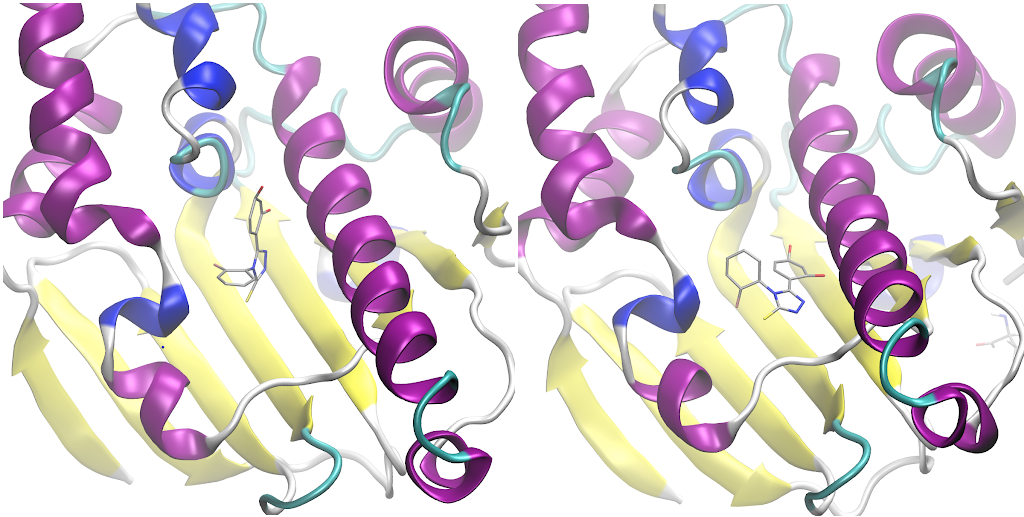
\includegraphics{images/htmd_analysis_bindingposes.png}

\subsection*{RMSF}
When considering the RMSF fluctuations greater than 1 Angstrom are worth
considering. These are seen near residue position 50, 110 and 160. Very
large fluctuations are seen for the final residues i.e.~the C-terminus.
Fairly common and no investigation is needed. The movement could be
related to binding or other motions.

% possibly RMSF fig but not really needed
\begin{figure}[h!]
  \caption{\csentence{RMSF for the protein.}
      RMSF}
\label{fig:rmsf}
      \end{figure}
%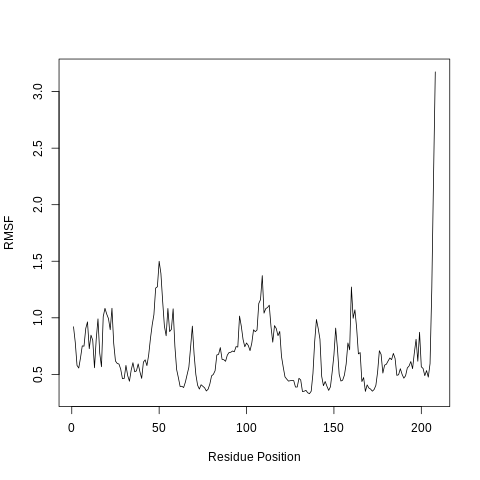
\includegraphics{images/htmd_analysis_rmsf.png}

\subsection*{PCA}

The first principal component (PC1) is most important accounting for
32.36\% of the variance (see PC1 vs PC2 and Eigenvalue rank plots). More
information on PCA can be found in the
\href{http://thegrantlab.org/bio3d/tutorials/trajectory-analysis}{BIO3D
tutorial}. The RMSF is in good correlation with PC1.

\begin{figure}[h!]
  \caption{\csentence{Principal Component Analysis.}
      PCA.}
\label{fig:rmsdligand}
      \end{figure}
%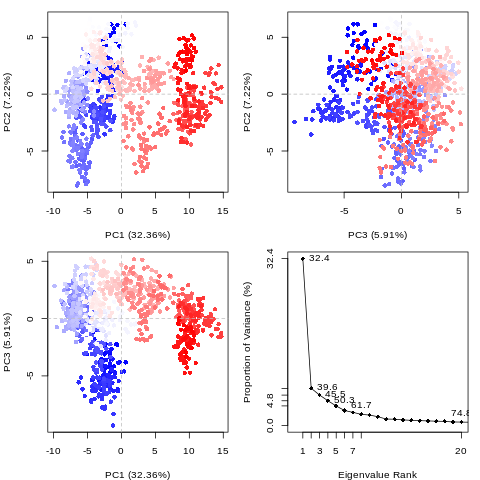
\includegraphics{images/htmd_analysis_pca.png}
%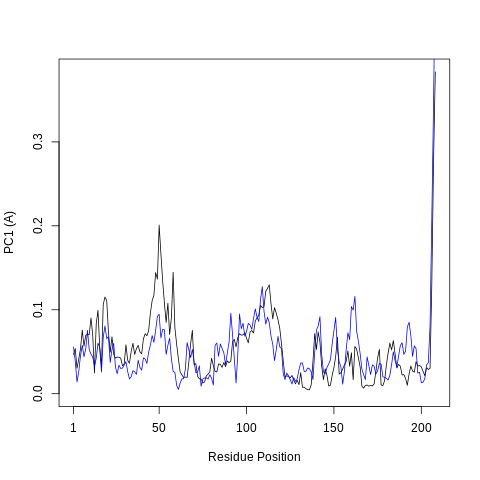
\includegraphics{images/htmd_analysis_pc1_rmsf.png}

\subsection*{Hydrogen bonding and further analysis}
The active site of this protein is quite hydrophobic. Only 1 hydrogen
bond is seen between the ligand and Hsp90, this is between Threonine 184
and the ligand. This hydogren bond is not persisent, the occupancy is
small, 0.20\%, the hydrogen is not present for most of the simulation
(according to the criteria for hydrogen bonding).
There are many alternative analyses that have not been considered for the sake of brevity. TODO consider adding another line or two.


\hypertarget{conclusion}{%
\section*{Conclusion}\label{conclusion}}

We provide an overview of ...



\section*{Section title}
Text for this section \ldots
\subsection*{Sub-heading for section}
Text for this sub-heading \ldots
\subsubsection*{Sub-sub heading for section}
Text for this sub-sub-heading \ldots
\paragraph*{Sub-sub-sub heading for section}
Text for this sub-sub-sub-heading \ldots
In this section we examine the growth rate of the mean of $Z_0$, $Z_1$ and $Z_2$. In


%%%%%%%%%%%%%%%%%%%%%%%%%%%%%%%%%%%%%%%%%%%%%%
%%                                          %%
%% Backmatter begins here                   %%
%%                                          %%
%%%%%%%%%%%%%%%%%%%%%%%%%%%%%%%%%%%%%%%%%%%%%%

\begin{backmatter}

\section*{Competing interests}
  The authors declare that they have no competing interests.

\section*{Author's contributions}
    Text for this section \ldots

\section*{Acknowledgements}
  Text for this section \ldots

\section*{Data and material availability}
  Data and materials are available on GitHub:
  TODO\ldots
%%%%%%%%%%%%%%%%%%%%%%%%%%%%%%%%%%%%%%%%%%%%%%%%%%%%%%%%%%%%%
%%                  The Bibliography                       %%
%%                                                         %%
%%  Bmc_mathpys.bst  will be used to                       %%
%%  create a .BBL file for submission.                     %%
%%  After submission of the .TEX file,                     %%
%%  you will be prompted to submit your .BBL file.         %%
%%                                                         %%
%%                                                         %%
%%  Note that the displayed Bibliography will not          %%
%%  necessarily be rendered by Latex exactly as specified  %%
%%  in the online Instructions for Authors.                %%
%%                                                         %%
%%%%%%%%%%%%%%%%%%%%%%%%%%%%%%%%%%%%%%%%%%%%%%%%%%%%%%%%%%%%%

% if your bibliography is in bibtex format, use those commands:
\bibliographystyle{bmc-mathphys} % Style BST file (bmc-mathphys, vancouver, spbasic).
\bibliography{bmc_article}      % Bibliography file (usually '*.bib' )
% for author-year bibliography (bmc-mathphys or spbasic)
% a) write to bib file (bmc-mathphys only)
% @settings{label, options="nameyear"}
% b) uncomment next line
%\nocite{label}

% or include bibliography directly:
% \begin{thebibliography}
% \bibitem{b1}
% \end{thebibliography}

%%%%%%%%%%%%%%%%%%%%%%%%%%%%%%%%%%%
%%                               %%
%% Figures                       %%
%%                               %%
%% NB: this is for captions and  %%
%% Titles. All graphics must be  %%
%% submitted separately and NOT  %%
%% included in the Tex document  %%
%%                               %%
%%%%%%%%%%%%%%%%%%%%%%%%%%%%%%%%%%%

%%
%% Do not use \listoffigures as most will included as separate files

\section*{Figures}
  \begin{figure}[h!]
  \caption{\csentence{Sample figure title.}
      A short description of the figure content
      should go here.}
      \end{figure}

\begin{figure}[h!]
  \caption{\csentence{Sample figure title.}
      Figure legend text.}
      \end{figure}


%%%%%%%%%%%%%%%%%%%%%%%%%%%%%%%%%%%
%%                               %%
%% Additional Files              %%
%%                               %%
%%%%%%%%%%%%%%%%%%%%%%%%%%%%%%%%%%%

\section*{Additional Files}
  \subsection*{Additional file 1 --- Sample additional file title}
    Additional file descriptions text (including details of how to
    view the file, if it is in a non-standard format or the file extension).  This might
    refer to a multi-page table or a figure.

  \subsection*{Additional file 2 --- Sample additional file title}
    Additional file descriptions text.


\end{backmatter}
\end{document}
